\documentclass[11pt]{article}
\usepackage[margin=0.7in]{geometry}
\usepackage{booktabs}
\usepackage{pgfplots}
\pgfplotsset{compat=1.18}
\usepackage{xcolor}
\definecolor{cQLIKE}{HTML}{0072B2}
\definecolor{cHMSE}{HTML}{009E73}
\definecolor{cMAE}{HTML}{56B4E9}
\definecolor{cMSE}{HTML}{E69F00}
\definecolor{cOOSR2}{HTML}{D55E00}
\begin{document}

\begin{table}[t]
\centering
\caption{Every-bar (refit $=1$) exogenous-bucket battery vs.\ the HAR baseline. Train window
1000 trading days; fixed COVID-inclusive evaluation window \textbf{Jan.\ 2018 -- May 2025}
($n = 74{,}934$ thirty-minute bars; 1{,}843 trading days; identical rows for every cell); best
penalty per bucket selected by QLIKE; HAR block unpenalized (OLS via Frisch--Waugh--Lovell).
DM $=$ Diebold--Mariano test on per-bar QLIKE loss vs.\ HAR-only, reported as ($t$, $p$): the
DM statistic is the $t$-ratio of the mean loss differential to its Newey--West HAC standard
error (Harvey--Leybourne--Newbold small-sample correction), with two-sided $p$-value.
The $90\%$ model confidence set contains ALL buckets alone;
every other bucket is eliminated. Raw-variance MSE and OOS-$R^2$ are dominated by a small number
of COVID bars; QLIKE, HMSE and MAE are the level-robust rankers.}
\vspace{4pt}
\footnotesize
\setlength{\tabcolsep}{4pt}
\begin{tabular}{@{}llccccccc@{}}
\toprule
exogenous bucket & penalty & QLIKE & MAE & MSE & OOS-$R^2$ & MZ-$\beta$ & MZ-$R^2$ & DM vs.\ HAR ($t$, $p$) \\
\midrule
\textbf{ALL buckets} & ridge $\alpha{=}30$ & \textbf{0.14265} & $1.213 \times 10^{-6}$ & $4.571 \times 10^{-11}$ & 0.6969 & 0.902 & 0.7058 & $-13.0$, $1.2 \times 10^{-38}$ \\
implied\_vol (VIX/VVIX) & ridge $\alpha{=}1$ & 0.14669 & $1.236 \times 10^{-6}$ & $4.558 \times 10^{-11}$ & 0.6978 & 0.907 & 0.7057 & $-8.7$, $2.3 \times 10^{-18}$ \\
moments & ridge $\alpha{=}1000$ & 0.14678 & $1.246 \times 10^{-6}$ & $4.624 \times 10^{-11}$ & 0.6935 & 0.879 & 0.7074 & $-7.5$, $4.6 \times 10^{-14}$ \\
liquidity & ridge $\alpha{=}1$ & 0.14679 & $1.250 \times 10^{-6}$ & $4.599 \times 10^{-11}$ & 0.6951 & 0.892 & 0.7060 & $-10.8$, $3.8 \times 10^{-27}$ \\
sentiment & enet $\alpha{=}10^{-3}$, $\ell_1{=}0.6$ & 0.14726 & $1.250 \times 10^{-6}$ & $4.484 \times 10^{-11}$ & \textbf{0.7027} & 0.901 & 0.7120 & $-8.2$, $2.9 \times 10^{-16}$ \\
market\_vw & enet $\alpha{=}10^{-3}$, $\ell_1{=}0.2$ & 0.14744 & $1.253 \times 10^{-6}$ & $4.558 \times 10^{-11}$ & 0.6978 & 0.891 & 0.7091 & $-8.7$, $4.5 \times 10^{-18}$ \\
market\_ew & ridge $\alpha{=}1000$ & 0.14758 & $1.257 \times 10^{-6}$ & $4.593 \times 10^{-11}$ & 0.6955 & 0.889 & 0.7071 & $-9.3$, $1.0 \times 10^{-20}$ \\
vol\_demand & enet $\alpha{=}10^{-3}$, $\ell_1{=}0.6$ & 0.14822 & $1.259 \times 10^{-6}$ & $4.553 \times 10^{-11}$ & 0.6982 & 0.900 & 0.7075 & $-6.2$, $5.0 \times 10^{-10}$ \\
\emph{HAR-only (baseline)} & none (OLS) & 0.14863 & $1.262 \times 10^{-6}$ & $4.545 \times 10^{-11}$ & 0.6987 & 0.898 & 0.7084 & (baseline) \\
\bottomrule
\end{tabular}
\end{table}

\begin{table}[t]
\centering
\caption{Intra-bucket bundle-combination factorial ($2^8$ over the stage-1 surviving bundles;
a bundle $=$ one variable's six-lag moving-average ladder plus its availability indicator).
Model: ridge $\alpha = 1$ on the square-root target with the RV-HAR ladder and intraday hour
dummies always included; every-bar refit. Primary window $tw = 48{,}000$ bars (1{,}000 trading
days): evaluation \textbf{Oct.\ 9, 2008 -- Apr.\ 30, 2024} ($n = 198{,}059$ bars). Replicate
window $tw = 144{,}000$ (3{,}000 days): evaluation \textbf{Apr.\ 25, 2016 -- Apr.\ 30, 2024}
($n = 102{,}059$ bars); its QLIKE level is not comparable across windows (different evaluation
spans) --- the ranking and DM are. DM ($t$-ratio, two-sided $p$; as in Table 1) is vs.\ the
HAR-baseline cell of the same window.
QLIKE levels here are not comparable to Table 1: this panel is the raw research build (no diurnal
adjustment or rank transform; overnight bars included), so the bundle gains include intraday
seasonality that Table 1's cache removes by construction --- within-table rankings and DM are the
deliverable. Exact factorial main effects on QLIKE, mean(bundle on) $-$ mean(bundle off) over
all $2^8$ cells ($tw48$k/$tw144$k): absret $-0.199$/$-0.257$; volume $-0.108$/$-0.063$; vvix $-0.023$/$-0.014$; sentcount $-0.011$/$+0.003$; vdem\_all $-0.010$/$+0.000$; attention $-0.010$/$+0.002$; vdem\_spx $-0.009$/$+0.001$; bipow $-0.000$/$-0.000$.
Largest first-order (two-way) interaction effects, same convention (positive $=$ partial
redundancy: the joint gain is less than additive): absret$\times$volume $+0.094$/$+0.064$; absret$\times$vvix $+0.020$/$+0.010$; volume$\times$vvix $+0.014$/$-0.005$.}
\vspace{4pt}
\scriptsize
\setlength{\tabcolsep}{2.5pt}
\begin{tabular}{@{}lccccccc@{}}
\toprule
& \multicolumn{5}{c}{$tw = 48{,}000$ (2008--2024)} & \multicolumn{2}{c}{$tw = 144{,}000$ (2016--2024)} \\
\cmidrule(lr){2-6}\cmidrule(l){7-8}
bundle combination & QLIKE & MAE & OOS-$R^2$ & MZ-$R^2$ & DM vs.\ HAR ($t$, $p$) & QLIKE & DM \\
\midrule
\multicolumn{8}{@{}l}{\emph{Main effects: the eight single-bundle cells (one bundle added to HAR), ranked by QLIKE}} \\
\midrule
absret & 0.38950 & $1.930 \times 10^{-6}$ & 0.3742 & 0.4592 & $-37.3$, $< 10^{-300}$ & 0.38686 & $-58.8$ \\
volume & 0.50567 & $2.561 \times 10^{-6}$ & 0.2159 & 0.2408 & $-31.3$, $1.6 \times 10^{-214}$ & 0.57475 & $-44.9$ \\
vvix & 0.68515 & $2.912 \times 10^{-6}$ & 0.1257 & 0.1731 & $-12.2$, $2.1 \times 10^{-34}$ & 0.66325 & $-23.9$ \\
sentcount & 0.71939 & $3.001 \times 10^{-6}$ & 0.0900 & 0.1099 & $-11.9$, $1.8 \times 10^{-32}$ & 0.69639 & $-7.1$ \\
vdem\_all & 0.72088 & $2.948 \times 10^{-6}$ & 0.0835 & 0.1117 & $-14.7$, $6.2 \times 10^{-49}$ & 0.68742 & $-8.4$ \\
attention & 0.72629 & $3.012 \times 10^{-6}$ & 0.0903 & 0.1111 & $-10.0$, $2.0 \times 10^{-23}$ & 0.68812 & $-8.4$ \\
vdem\_spx & 0.73552 & $3.009 \times 10^{-6}$ & 0.0817 & 0.1059 & $-12.6$, $1.3 \times 10^{-36}$ & 0.67324 & $-13.0$ \\
bipow & 0.78314 & $3.106 \times 10^{-6}$ & 0.0763 & 0.1004 & $-6.2$, $4.3 \times 10^{-10}$ & 0.72567 & $-2.1$ \\
\midrule
\multicolumn{8}{@{}l}{\emph{Selected combination cells: best by QLIKE; best-six of the P\&L factorial; the full set}} \\
\midrule
absret, volume, vdem\_all, bipow & \textbf{0.34598} & $1.862 \times 10^{-6}$ & 0.3629 & 0.4291 & $-40.9$, $< 10^{-300}$ & 0.36599 & $-61.1$ \\
absret, volume, vdem\_all, vvix, sentcount, attention & 0.35237 & $1.862 \times 10^{-6}$ & 0.3771 & 0.4400 & $-39.3$, $< 10^{-300}$ & 0.37061 & $-58.5$ \\
all eight bundles & 0.35156 & $1.862 \times 10^{-6}$ & 0.3774 & 0.4399 & $-39.4$, $< 10^{-300}$ & 0.37023 & $-58.1$ \\
\midrule
\emph{HAR ladder $+$ hour dummies (baseline)} & 0.78614 & $3.109 \times 10^{-6}$ & 0.0758 & 0.1002 & (baseline) & 0.72675 & (baseline) \\
\bottomrule
\end{tabular}
\end{table}

\begin{figure}[t]
\centering
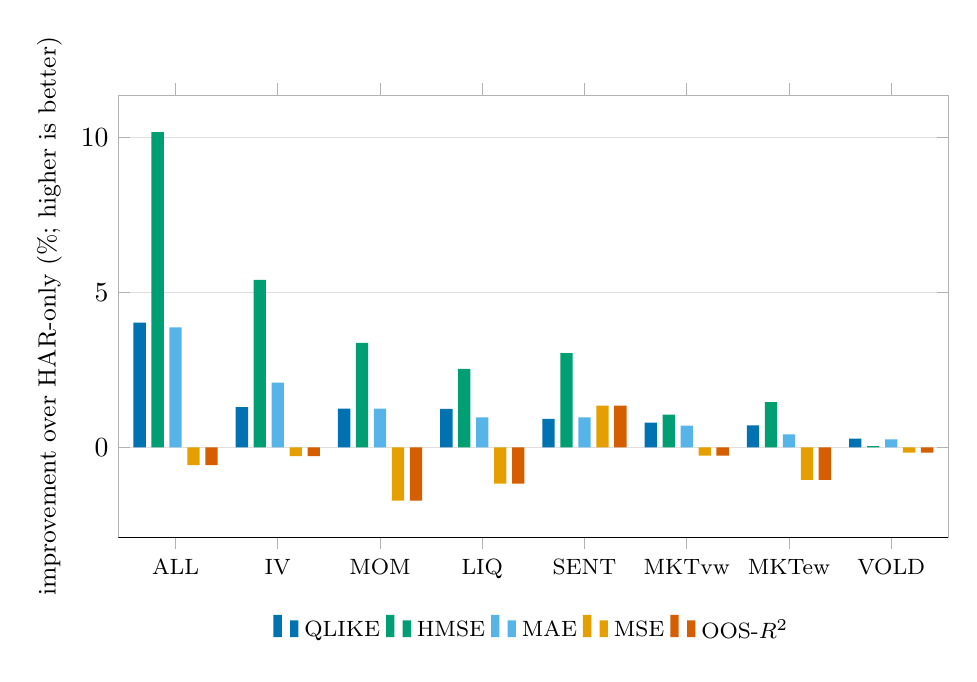
\begin{tikzpicture}
\begin{axis}[
  ybar, bar width=4.5pt,
  width=\textwidth, height=7.2cm,
  symbolic x coords={ALL,IV,MOM,LIQ,SENT,MKTvw,MKTew,VOLD},
  xtick=data, x tick label style={font=\footnotesize},
  enlarge x limits=0.08,
  ymajorgrids, grid style={gray!25},
  axis line style={gray!60}, tick style={gray!60},
  ylabel={improvement over HAR-only (\%; higher is better)},
  ylabel style={font=\small},
  legend style={at={(0.5,-0.16)}, anchor=north, legend columns=5, font=\footnotesize, draw=none},
  every axis plot/.append style={draw opacity=0},
]
\addplot+[ybar, fill=cQLIKE, draw=white, line width=0.3pt] coordinates {(ALL,4.02) (IV,1.30) (MOM,1.25) (LIQ,1.24) (SENT,0.92) (MKTvw,0.80) (MKTew,0.71) (VOLD,0.28)};
\addplot+[ybar, fill=cHMSE, draw=white, line width=0.3pt] coordinates {(ALL,10.17) (IV,5.40) (MOM,3.37) (LIQ,2.53) (SENT,3.04) (MKTvw,1.06) (MKTew,1.46) (VOLD,0.04)};
\addplot+[ybar, fill=cMAE, draw=white, line width=0.3pt] coordinates {(ALL,3.87) (IV,2.09) (MOM,1.25) (LIQ,0.97) (SENT,0.97) (MKTvw,0.70) (MKTew,0.42) (VOLD,0.26)};
\addplot+[ybar, fill=cMSE, draw=white, line width=0.3pt] coordinates {(ALL,-0.57) (IV,-0.28) (MOM,-1.72) (LIQ,-1.17) (SENT,1.35) (MKTvw,-0.27) (MKTew,-1.05) (VOLD,-0.17)};
\addplot+[ybar, fill=cOOSR2, draw=white, line width=0.3pt] coordinates {(ALL,-0.57) (IV,-0.28) (MOM,-1.72) (LIQ,-1.17) (SENT,1.35) (MKTvw,-0.27) (MKTew,-1.05) (VOLD,-0.17)};
\draw[black, thin] (rel axis cs:0,0.0) -- (rel axis cs:1,0.0);
\legend{QLIKE, HMSE, MAE, MSE, OOS-$R^2$}
\end{axis}
\end{tikzpicture}
\caption{Every metric of Table 1 mapped to one comparable scale: fractional improvement over
HAR-only, sign-oriented so that larger is better (the OOS-$R^2$ improvement is scaled by
$1-R^2_{\mathrm{HAR}}$). The level-robust metrics (QLIKE, HMSE, MAE) agree --- the full bucket
set wins decisively (DM $p = 1.2 \times 10^{-38}$) --- while raw-variance MSE and OOS-$R^2$
collapse toward zero or reverse sign, reflecting COVID-bar domination rather than forecast skill.}
\end{figure}

\end{document}
